\documentclass[12pt]{beamer}
\usepackage{../Estilos/BeamerMAF}
\input{../Preambulos/preambulo_Beamer_Warsaw_seahorse}
\makeatletter
\setbeamertemplate{footline}
{
  \leavevmode%
  \hbox{%
  \begin{beamercolorbox}[wd=.333333\paperwidth,ht=2.25ex,dp=1ex,center]{section in foot}%
    \usebeamerfont{section in foot} \insertsection
  \end{beamercolorbox}%
  \begin{beamercolorbox}[wd=.333333\paperwidth,ht=2.25ex,dp=1ex,center]{subsection in foot}%
    \usebeamerfont{subsection in foot}  \insertsubsection
  \end{beamercolorbox}%
  \begin{beamercolorbox}[wd=.333333\paperwidth,ht=2.25ex,dp=1ex,right]{date in head/foot}%
    \usebeamerfont{date in head/foot} {Material adicional} \hspace*{2em}
    \insertframenumber{} / \inserttotalframenumber \hspace*{2ex} 
  \end{beamercolorbox}}%
  \vskip0pt%
}
\makeatother
\makeatletter
\patchcmd{\beamer@sectionintoc}{\vskip1.5em}{\vskip0.8em}{}{}
\makeatother

\title{\large{Más Ejercicios}}
\subtitle{Funciones Gamma y Beta}
\author{M. en C. Gustavo Contreras Mayén}
\date{}
\institute{Facultad de Ciencias - UNAM}
\titlegraphic{\includegraphics[width=1.75cm]{../Imagenes/escudo-facultad-ciencias}\hspace*{4.75cm}~%
   \includegraphics[width=1.75cm]{../Imagenes/escudo-unam}
}
\setbeamertemplate{navigation symbols}{}
\begin{document}
\maketitle
\fontsize{14}{14}\selectfont
\spanishdecimal{.}
\section*{Contenido}
\frame[allowframebreaks]{\tableofcontents[currentsection, hideallsubsections]}

\section{Batería de ejercicios}
\frame{\tableofcontents[currentsection, hideothersubsections]}

\begin{frame}
\frametitle{Uso de identidades}
En los siguientes ejercicios se ocuparán las identidades que se han enlistado en los materiales de trabajo, y que algunas se han demostrado en un video previo.
\end{frame}

\subsection{Ejercicios Función Gamma}

\begin{frame}
\frametitle{Evaluación de integrales}
Evalúa la integral:
\begin{align*}
\int_{0}^{\frac{\pi}{2}} \sqrt{\cos \theta} \dd{\theta}
\end{align*}
\pause
En este tipo de integrales, ocupamos las expresiones que hemos revisado previamente.
\end{frame}
\begin{frame}
\frametitle{Completando la integral}
Agregamos un \enquote{uno} en el integrado: de la forma $\frac{2}{2}$ y $\sin^{0} \theta$, así que:
\pause
\begin{eqnarray*}
\int_{0}^{\frac{\pi}{2}} \sqrt{\cos \theta} \dd{\theta} = \dfrac{1}{2} \scaleto{\int_{0}^{\frac{\pi}{2}}}{35pt} 2 \, \sin^{0} \theta \, \cos^{\frac{1}{2}} \theta \dd{\theta}
\end{eqnarray*}
\pause
Ocupamos la identidad (que ya se demostró):
\begin{align*}
B(x, y) = \int_{0}^{\frac{\pi}{2}} 2 \, \sin^{2x-1} \theta \, \cos^{2y-1} \theta \dd{\theta}
\end{align*}    
\end{frame}
\begin{frame}
\frametitle{Solución}
Entonces tenemos que $2 \, x - 1 = 0$ y $2 \, y - 1 = 1/2$, por lo que:
\pause
\begin{eqnarray}
&{}& \int_{0}^{\frac{\pi}{2}} \sqrt{\cos \theta} \dd{\theta} = \dfrac{1}{2} B\left( \dfrac{1}{2}, \dfrac{3}{4} \right) \nonumber \\[0.5em] \pause
&=& \dfrac{\Gamma \left( \dfrac{1}{2} \right) \, \Gamma \left( \dfrac{3}{4} \right)}{2 \, \Gamma \left( \dfrac{5}{4} \right)} = \pause \dfrac{\sqrt{\pi} \, \Gamma \left( \dfrac{3}{4} \right)}{2 \, \Gamma \left( \dfrac{5}{4} \right)} \label{eq:ecuacion_02_14_01}
\end{eqnarray}
\end{frame}
\begin{frame}
\frametitle{Uso de otra identidad}
Haremos uso de la siguiente identidad:
\begin{align*}
\Gamma (p) \, \Gamma(1 - p) = \dfrac{\pi}{\sin p \pi} \hspace{1.5cm} p \mbox{ no entero}
\end{align*}
\pause
Esta identidad se puede demostrar ocupando otras relaciones tanto para la función Gamma y Beta.
\end{frame}
\begin{frame}
\frametitle{Continuamos con la solución}
Ahora ocupamos la identidad anterior para obtener un resultado que nos servirá para con la solución:
\begin{eqnarray*}
\Gamma \left( \dfrac{1}{4} \right) \, \Gamma \left( \dfrac{3}{4} \right) = \pause \dfrac{\pi}{\sin \left( \dfrac{1}{4}\right) \pi} = \pause \pi \sqrt{2}
\end{eqnarray*}
\pause
Por lo tanto:
\begin{align*}
\Gamma \left( \dfrac{3}{4} \right) = \dfrac{\pi \sqrt{2}}{\Gamma \left(\dfrac{1}{4} \right)}
\end{align*}
\end{frame}
\begin{frame}
\frametitle{Simplificando el denominador}
El denominador que tenemos en nuestra expresión, se simplifica de la siguiente forma:
\pause
\begin{align*}
\Gamma \left( \dfrac{5}{4} \right) = \dfrac{1}{4} \, \Gamma \left( \dfrac{1}{4} \right)
\end{align*}
\pause
Al sustituir estos resultados en la ec. (\ref{eq:ecuacion_02_14_01}), llegamos a:
\begin{align*}
\int_{0}^{\frac{\pi}{2}} \sqrt{\cos \theta} \dd{\theta} = \dfrac{(2 \, \pi)^{3/2}}{\left[ \Gamma \left( \dfrac{1}{4} \right) \right]^{2}} \hspace{1cm} \qed
\end{align*}
\end{frame}
\begin{frame}
\frametitle{Área dentro de una curva}
Calcula el área contenida dentro de la curva
\begin{align*}
x^{20} + y^{20} = a^{20}
\end{align*}
\pause
Para resolver este ejercicio, ocuparemos una identidad que ya se demostró anteriormente.
\end{frame}
\begin{frame}
\frametitle{La curva en cuestión}
Esta es una curva que es casi un cuadrado, donde el exponente común $b / c$ es un entero par bastante grande.
\begin{figure}[H]
  \centering
  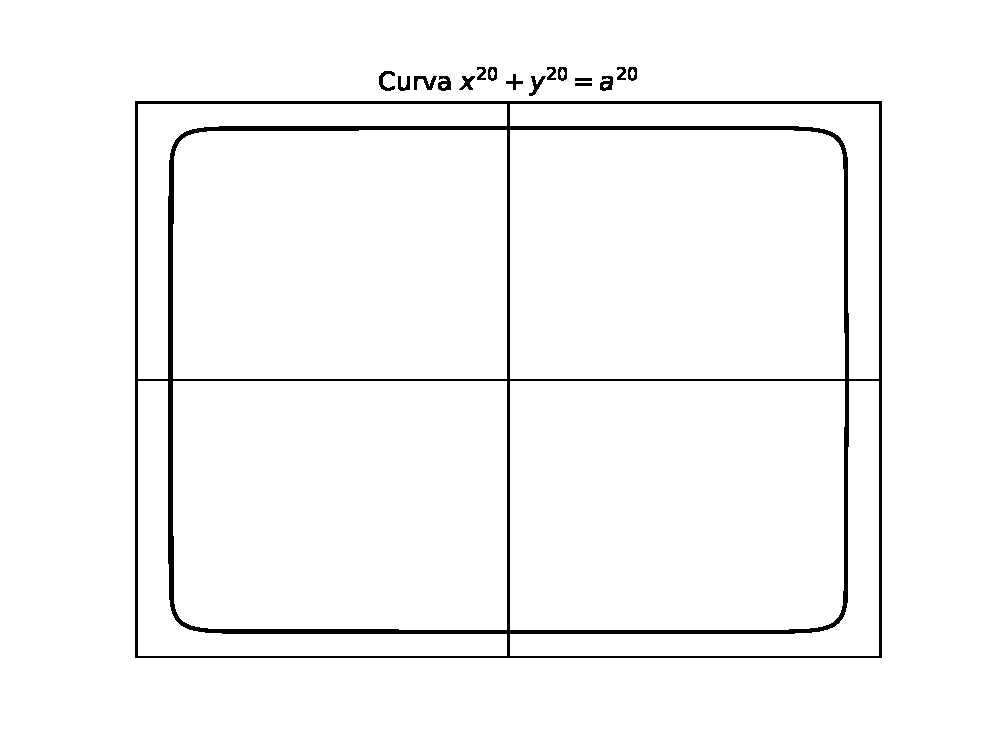
\includegraphics[scale=0.41]{Imagenes/plot_curva_estrella_03.eps}
\end{figure}
\end{frame}
\begin{frame}
\frametitle{Solución}
Ya se hizo la demostración de la solución general:
\begin{align*}
A = \dfrac{\mathlarger{\Gamma} \left( \dfrac{c}{b} \right) \, \mathlarger{\Gamma} \left( \dfrac{c}{b} \right)}{\mathlarger{\Gamma} \left( \dfrac{2 \, c}{b} \right)} \, \left( \dfrac{2 \, c \, a^{2}}{b} \right)
\end{align*}
Por lo que para la solución particular, ocupamos los valores de $b = 20$ y $c = 1$.
\end{frame}
\begin{frame}
\frametitle{Solución particular}
\begin{eqnarray*}
A &=& \dfrac{\mathlarger{\Gamma} \left( \dfrac{c}{b} \right) \mathlarger{\Gamma} \left( \dfrac{c}{b} \right)}{\mathlarger{\Gamma} \left( \dfrac{2 c}{b} \right)} \left( \dfrac{2 c a^{2}}{b} \right) = \pause \dfrac{\mathlarger{\Gamma} \left( \dfrac{1}{20} \right) \mathlarger{\Gamma} \left( \dfrac{1}{20} \right)}{\mathlarger{\Gamma} \left( \dfrac{2}{20} \right)} (2) \left( \dfrac{1}{20} \right) a^{2} \\[0.5em] \pause
&=& \dfrac{400 \, \mathlarger{\Gamma} \left( \dfrac{21}{20} \right) \mathlarger{\Gamma} \left( \dfrac{21}{20} \right)}{10 \, \mathlarger{\Gamma} \left( \dfrac{11}{10} \right)} (2) \left( \dfrac{1}{20} \right) a^{2} \\[0.5em] \pause
\end{eqnarray*}  
\end{frame}
\begin{frame}
\frametitle{Solución particular}
\begin{align*}
A \cong 4 \left[ \dfrac{(0.9735)(0.9735)}{0.9514} \right] \, a^{2}
\end{align*}  
\pause
La cantidad entre los corchetes a cuatro decimales es $0.9961$, Por lo tanto, la solución es:
\begin{align*}
A \cong 4 \, a^{2}
\end{align*}
\end{frame}
\begin{frame}
\frametitle{Extendiendo el resultado}
Demuestra que si el exponente $b/c$ en el problema anterior, es un valor par positivo $2 \, m$, el área dentro de la curva $A$ se acerca al límite $4 \, a^{2}$ cuando $m \to \infty$.
\end{frame}
\begin{frame}
\frametitle{Consideración}
Este resultado es lo que naturalmente esperamos al considerar la forma y posición de las curvas de la familia:
\begin{align*}
x^{2m} + y^{2m} = a^{2m}
\end{align*}
\end{frame}
\begin{frame}
\frametitle{Solución}
Como ya tenemos la solución general para el área dentro de la curva, ahora consideramos el límite cuando $m \to \infty$:
\begin{align*}
\lim_{m \to \infty} A = a^{2} \lim_{m \to \infty} \dfrac{\mathlarger{\Gamma} \left( \dfrac{1}{2 \, m} \right) \, \mathlarger{\Gamma} \left( \dfrac{1}{2 \, m} \right)}{m \, \mathlarger{\Gamma} \left( \dfrac{1}{m} \right)}
\end{align*}
\end{frame}
\begin{frame}
\frametitle{Ocupando una identidad}
Ocupamos la siguiente identidad:
\begin{align*}
\Gamma (x) = \dfrac{\Gamma (x + 1)}{x}
\end{align*}
De tal manera que:
\begin{eqnarray*}
\Gamma \left( \dfrac{1}{2 \, m} \right) &=& 2 \, m \, \Gamma \left( \dfrac{1}{2 \, m} + 1 \right) \\[0.5em] \pause
\Gamma \left( \dfrac{1}{m} \right) &=& m \, \Gamma \left( \dfrac{1}{m} + 1 \right)
\end{eqnarray*}
\end{frame}
\begin{frame}
\frametitle{Tomando el límite}
Acomodando los términos y llevando al límite cuando $m \to \infty$, se tiene que:
\begin{eqnarray*}
\lim_{m \to \infty} A &=& a^{2} \lim_{m \to \infty} \dfrac{2 m \mathlarger{\Gamma} \left( \dfrac{1}{2m} {+} 1 \right) \, 2 m \mathlarger{\Gamma} \left( \dfrac{1}{2m} {+} 1 \right)}{m m \, \mathlarger{\Gamma} \left( \dfrac{1}{m} {+} 1 \right)} = \\[0.5em] \pause 
&=& 4 \, a^{2} \, \Gamma(1) = \pause 4 \, a^{2} \hspace{1cm} \qed
\end{eqnarray*}
\end{frame}
  


\end{document}